\documentclass[12pt,a4paper]{article}

\usepackage{graphicx}
\usepackage{amsmath}
\usepackage{geometry}
\usepackage{xcolor}
\usepackage{array}

\geometry{margin=1in}

\begin{document}

%================ HEADER =================

\noindent
\begin{minipage}{0.6\textwidth}
    
\includegraphics[width=6cm]{Logo.png}
\end{minipage}
\begin{minipage}{0.4\textwidth}
    \raggedleft
    \textbf{Name:} Pavan Kumar KS\\
    \textbf{Batch:} COMETFWC044\\
    \textbf{Date:} 16 Feb 2026\\
\end{minipage}

\vspace{20pt}

\begin{center}
    \Large \textbf{Gate Question 2010 EE, Question No.52}
\end{center}

%==================================================
\section*{\textcolor{blue}{Question}}

\textbf{Linked Answer Questions}

\textbf{Statement for Linked Answer Questions 52 and 53:}

The following Karnaugh map represents a function $F$.

\vspace{0.4cm}

\begin{center}
\begin{tabular}{c|c c c c}
 & \multicolumn{4}{c}{$YZ$} \\
 & 00 & 01 & 11 & 10 \\
\hline
$X=0$ & 1 & 1 & 1 & 0 \\
$X=1$ & 0 & 0 & 1 & 0 \\
\end{tabular}
\end{center}

\vspace{0.4cm}

\textbf{Q.52} A minimized form of the function $F$ is:

\begin{enumerate}
\item[(A)] $F = \overline{X}Y + YZ$
\item[(B)] $F = XY + YZ$
\item[(C)] $F = \overline{X}\overline{Y} + \overline{Y}Z$
\item[(D)] $F = X\overline{Y} + \overline{Y}Z$
\end{enumerate}

\vspace{0.3cm}
\textbf{Correct Answer: (B)}

%==================================================
\section*{\textcolor{blue}{Question Analysis}}

From the K-map:

\[
F = \sum m(0,1,3,7)
\]

Grouping gives:

\[
F = XY + YZ
\]

%==================================================
\section*{\textcolor{blue}{Truth Table}}

\begin{center}
\begin{tabular}{|c|c|c|c|}
\hline
X & Y & Z & F \\
\hline
0 & 0 & 0 & 1 \\
0 & 0 & 1 & 1 \\
0 & 1 & 0 & 0 \\
0 & 1 & 1 & 1 \\
1 & 0 & 0 & 0 \\
1 & 0 & 1 & 0 \\
1 & 1 & 0 & 0 \\
1 & 1 & 1 & 1 \\
\hline
\end{tabular}
\end{center}

%==================================================
\section*{\textcolor{blue}{Hardware Implementation}}

The minimized expression is implemented using Arduino UNO and a 7-segment display.  
Inputs X, Y, Z are manually connected.  
Output F is displayed as 0 or 1.

%==================================================
\section*{\textcolor{blue}{Required Components}}

\begin{itemize}
\item Arduino UNO
\item Breadboard
\item 7-Segment Display (Common Cathode)
\item 220$\Omega$ Resistor
\item Jumper Wires
\end{itemize}

%==================================================
\section*{\textcolor{blue}{Pin Connections}}

\textbf{Inputs}

\begin{center}
\begin{tabular}{|c|c|}
\hline
Input & Arduino Pin \\
\hline
X & 2 \\
Y & 3 \\
Z & 4 \\
\hline
\end{tabular}
\end{center}

Open = 1  

Connect to GND = 0  

\vspace{10pt}

\textbf{7-Segment Connections}

\begin{center}
\begin{tabular}{|c|c|}
\hline
Segment & Arduino Pin \\
\hline
a & 5 \\
b & 6 \\
c & 7 \\
d & 8 \\
e & 9 \\
f & 10 \\
g & 11 \\
\hline
\end{tabular}
\end{center}

Common Cathode $\rightarrow$ 220$\Omega$ $\rightarrow$ GND

%==================================================
\section*{\textcolor{blue}{Logic Description}}

\[
F = XY + YZ
\]

If $F=1$ → Display 1  

If $F=0$ → Display 0  

%==================================================
\section*{\textcolor{blue}{Code Uploading Steps}}

\begin{enumerate}
    \item Create a Platform IO project.
    \item Write the code in main.cpp inside the src folder.
    \item Run the PIO project with command "pio run". It will compile the code and create a .hex file.
    \item Copy the .hex file to the ArduinoDroid folder.
    \item Connect the Arduino UNO to mobile using OTG cable.
    \item Upload the .hex file using "Upload Precompiled" option.
    \item Observe the output and verify the expression.
\end{enumerate}


\section*{\textcolor{blue}{Experimental Truth Table}}

The experimentally verified truth table is shown below:

\begin{center}
\begin{tabular}{|c|c|c|c|}
\hline
X & Y & Z & F (Observed) \\
\hline
0 & 0 & 0 & 1 \\
0 & 0 & 1 & 1 \\
0 & 1 & 0 & 0 \\
0 & 1 & 1 & 1 \\
1 & 0 & 0 & 0 \\
1 & 0 & 1 & 0 \\
1 & 1 & 0 & 0 \\
1 & 1 & 1 & 1 \\
\hline
\end{tabular}
\end{center}

The experimental results match the theoretical expression:

\[
F = XY + YZ
\]

\vspace{0.5cm}

\begin{figure}
\centering
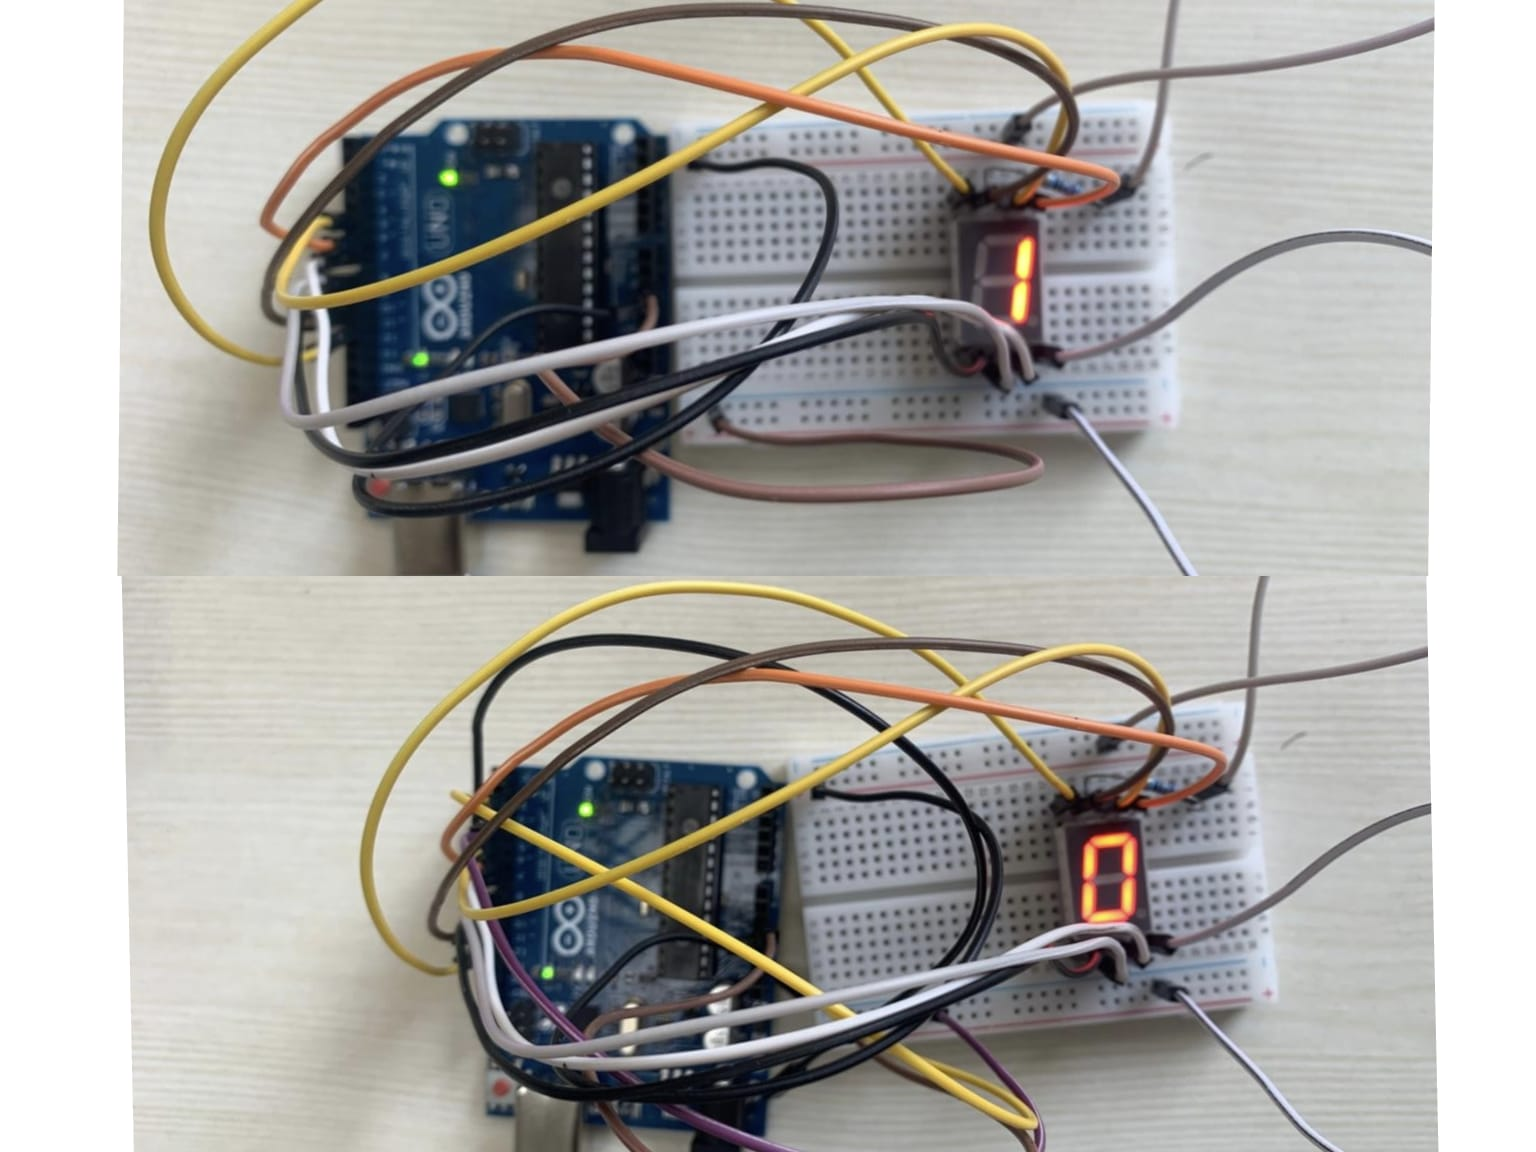
\includegraphics[width=0.9\textwidth]{experiment_photo.jpg}
\end{figure}
%==================================================
\section*{\textcolor{blue}{Conclusion}}

The minimized Boolean expression of the given function is:

\[
F = XY + YZ
\]

This matches Option (B).  
Experimental output matches theoretical results.

\end{document}
